%% MIS-749 Final Project
%% ----------------------------------------------------------------------
% Loading packages
\documentclass[stu, floatsintext, 11pt]{apa7}
\usepackage{lipsum}
\usepackage[american]{babel}
\usepackage{csquotes}
\usepackage[style=apa,sortcites=true,sorting=nyt,backend=biber]{biblatex}
\usepackage{hyperref}
\hypersetup{colorlinks,urlcolor=blue}
\usepackage{makecell}

% Bibliography
\DeclareLanguageMapping{american}{american-apa}
\addbibresource{bibliography.bib}

% TITLE PAGE
\title{Biodiversity's Effect on the Number of Visitors at National Parks}
\author{Elizabeth Fabio}
\affiliation{Department of Management Information Systems, San Diego State University}
\course{MIS-749: Business Analytics}
\professor{Dr. Aaron Elkins}
\duedate{May 12, 2020}

\begin{document}
\maketitle

% SECTION 1: EXECUTIVE SUMMARY
\section{Executive Summary}
U.S. National Parks can get up to 91 million recreational visits each year. Other than the beautiful landmarks, a lot of people visit the parks in hope to scout some wildlife. The National Park Service (NPS) keeps a detailed report of all their species along with the number of visitors for each year. With the data taken from Kaggle and the NPS site, I wanted to see if the biodiversity in these parks has an effect on the number of visitors. \\

The visitor count of each park was filtered for the year 2016 only since the species collection data was taken around that time. There are about 119,000 recorded species with 18 different features. Only seven of these features were further modeled since those qualitative variables had too many categories (at least more than 30) that would add complexity to the model (refer to Table \ref{tab:species_parks_v2}). Also, a subset of data was analyzed as well, which focused on the attributes of each national park. These attributes include the number of species and size in acres as the independent variables and the number of visitors as the dependent variable (refer to Table \ref{tab:species_parks_subset}). The reason why this subset was not incorporated into the species biodiversity dataset is that it would add weight to the number of species attribute when the row is only about one particular species. It was easier to breakdown the model for better analysis and interpretation. \\

The following models performed on the biodiversity dataset are linear regression, dimensionality reduction (principal component regression (PCR) and partial least squares (PLS)), feature selection (lasso and ridge regression), general additive model (GAM) smoothing splines, and random forest. As for the park subset data, the only models performed are linear regression, kNN, and GAM smoothing spline. After splitting these datasets into training and testing sets, a 10-fold cross validation was performed to find the best parameters to apply on the models in the testing set. \\

The RMSE and $R^2$ from the testing set showed linear regression as a good all-around model to use. It even performed fairly well on the biodiversity dataset that had a lot dimensionality. Also, the random forest model, as expected, had a good performance since it can manage non-linear datasets and qualitative variables well. For the park subset data, the kNN unexpectedly, came out to be the best model. The model can be sensitive when choosing the right number of neighbors, but after optimizing the parameter through cross-validation, the model overcame the bias-variance tradeoff. \\

Focusing on a handful of national parks and incorporating  features other than biodiversity can help determine what influences the number of visitors to these national parks. This knowledge is important for NPS to know so they can protect wildlife, maintain crowd control, and preserve these parks overall.

For these datasets, I used Python and R as my main tools for pre-processing and modeling. The CSV files and code can be found in the my GitHub repository, \href{https://github.com/ohkaaaaay/NP_Biodiversity}{NP\_Biodiverity}.

% SECTION 2: DISCOVERY AND DATA
\section{Discovery and Data Preparation}

%-----------------------------------------------------------------
% SUBSECTION 2.1: BIODIVERSITY IN NP DATASET
\subsection{Biodiversity in National Parks Dataset}
The bulk of the data originated from Kaggle's dataset called \href{https://www.kaggle.com/nationalparkservice/park-biodiversity}{Biodiversity in National Parks}. This dataset contains two CSV files. One file, called parks.csv, lists general national park (NP) information such as the number of acres and and the state where its located. Another file, called species.csv, lists each species with a variety of attributes ranging from its occurrence in the park to its scientific name. \\

Table \ref{tab:parks} and \ref{tab:species} displays the metadata of these two CSV files. It lists the type of data (quantitative or qualitative) along with its description. The parks.csv file has 56 rows representing the 56 parks in the U.S. at that time. The species.csv file is a much larger dataset containing 119,248 rows. The reason why this dataset was selected for modeling is to observe if species at a national park has an effect on the number of visitors.

% TABLE 1: Metadata of parks.csv
\begin{table}[h!]
    \centering
    \caption{parks.csv Metadata}
    \begin{tabular}{c c c}
    \hline
    \textbf{Attributes} & \textbf{Type} & \textbf{Description} \\
    \hline
    Park Code & Qualitative & Unique identifier for NP \\
    Park Name & Qualitative & NP name \\
    State & Qualitative & State where the NP is located \\
    Acres & Quantitative & Size of the NP \\
    Latitude & Quantitative & Latitude of where the NP is located \\ 
    Longitude & Quantitative & Longitude of where the NP is located \\
    \hline
    \end{tabular}
    \label{tab:parks}
\end{table}

% TABLE 2: Metadata of species.csv
\begin{table}[h!]
    \centering
    \caption{parks.csv Metadata}
    \resizebox{\textwidth}{!}{
    \begin{tabular}{c c c}
    \hline
    \textbf{Attributes} & \textbf{Type} & \textbf{Description} \\
    \hline
    Species ID & Qualitative & Unique identifier of species \\ 
    Park Name & Qualitative & NP name \\
    Category & Qualitative & Class name of a species  \\
    Order & Qualitative & Order name of a species \\
    Family & Qualitative & Family name of a species \\
    Scientific Name & Qualitative & Scientific name of the species \\
    Common Names & Qualitative & Commonly used names of that species \\
    Record Status & Qualitative & Determines if the dataset is active to use \\
    Occurrence & Qualitative & Status of the species presence in the park \\
    Nativeness & Qualitative & Native status at the park \\
    Abundance & Qualitative & How often the species seen at the park \\
    Seasonality & Qualitative & When the species is seen at the park \\
    Conservation Status & Qualitative & \makecell{Conservation status based on the International \\ Union for Conservation of Nature (IUCN)} \\ 
    \hline
    \end{tabular}
    }
    \label{tab:species}
\end{table}

%-----------------------------------------------------------------
% SUBSECTION 2.2: ANNUAL VISITATION & RECORD YEAR BY PARK DATASET
\subsection{Annual Visitation and Record Year by Park (1904 - 2020) Dataset}
The \href{https://irma.nps.gov/STATS/SSRSReports/National\%20Reports/Annual\%20Visitation\%20and\%20Record\%20Year\%20by\%20Park\%20(1904\%20-\%20Last\%20Calendar\%20Year}{Annual Visitation \& Record Year By Park dataset}, saved as a CSV filed called Annual\_NP\_Visitation.csv, lists the number of recreational visitors for each national park from 1904 to 2020. The reason why the year 2016 was filtered versus the most recent available data from 2020 is because the biodiversity dataset was downloaded from the National Park Services (NPS) website on January 6, 2017. Thus, the biodiversity dataset most likely contains the latest update from 2016.

%-----------------------------------------------------------------
% SUBSECTION 2.3: PRE-PROCESSING IN PYTHON
\subsection{Pre-Processing in Python}
In this pre-processing step, the goal is to join all the tables from the parks.csv, the species.csv, and the Annual\_NP\_Visitation.csv. Python was used along with the Pandas package in Jupyter Notebook to perform the following steps:
\begin{enumerate}
    \item Replace "NP" to "National Park" in the park name column of the annual visitors table so it can have the same format as the park name column in parks.csv. This will make sure that the two tables merge appropriately.
    \item Filter the annual visitors table to only the year 2016 since the other years are not needed.
    \item Merge the TRV, or Total Recorded Visitors, column from the 2016 annual visitors table to the species table by the park name.
    \item Join the newly merged visitors-park table to the species table.
    \item Save this new table as a CSV file called species\_parks.csv.
\end{enumerate}

The code on each of these steps is recorded in the IPython notebook called \href{https://github.com/ohkaaaaay/NP_Biodiversity/blob/main/NP_Bio_Data_Preproccesing_Part1.ipynb}{NP\_Bio\_Data\_Preproccesing\_Part1.ipynb}.\\

%-----------------------------------------------------------------
% SUBSECTION 2.4: PRE-PROCESSING IN R
\subsection{Pre-Processing in R}
In this step, two tables are created for further modeling. One table (species\_parks\_subset.csv) list each national park along with its number of visitors in 2016, its species count, and its size (in acres). The other table (species\_parks\_v2.csv) contains the majority of the species.csv columns. An important distinction between these two tables is that one table lists attributes about each national park and the other lists the attributes of each species. These two tables merged together would not work well in modeling because they would add unnecessary weight to certain attributes like the species count. \\

Another pre-processing step taken is addressing the NA values in the species\_parks\_subset table for the visitor count column. This issue is due to differences in several national park names. For instance, the Sequoia and Kings Canyon National Parks row showed zero visitors because the annual visitors table and the parks table did not merge properly. From here the NA values would be replaced with the actual visitor count. \\

For the code on this section's data pre-processing, refer to the R script called \href{https://github.com/ohkaaaaay/NP_Biodiversity/blob/main/NP_Bio_Data_Preproccesing_Part2.R}{NP\_Bio\_Data\_Preproccesing\_Part2.R}.

%-----------------------------------------------------------------
% SECTION 3: MODEL PLANNING AND BUILDING
\section{Model Planning and Building}
In analyzing the biodiversity and recreational visits at national parks, the goal was to find underlying trends between certain types of species and the number of visitors. To stick to this goal, the regression model was split into two methods since one dataset is centered around the number of species at each national park and the other dataset is centered around specific species attributes. \\

There are some initial concerns before building the model. One concern is the species\_parks\_subset dataset has only 56 observation. However, there are only 56 national parks. So finding more values to use for modeling is impossible. The best approach at this point is to keep this concern in mind. \\

Another concern to consider before building the model is the number of categories in some of the qualitative attributes from species\_parks\_v2. For example, the species' family name, order name, and scientific name would be too specific for regression modeling and it could lead to overfitting. In working around this, the columns with a large number of unique categories were removed for modeling.

% SUBSECTION 3.1: SPECIES & ACRES
\subsection{Number of Species and Acre Size Analysis on Visitor Count}
The R script, \href{https://github.com/ohkaaaaay/NP_Biodiversity/blob/main/Species_Acres_Modeling.R}{Species\_Acres\_Modeling.R}, contains all the code for modeling species\_parks\_subset. Table \ref{tab:species_parks_subset} shows the variables used for the following regression models: 
\begin{enumerate}
    \item Linear Regression
    \item General Additive Model (GAM) Smoothing Splines
    \item k-Nearest Neighbors (kNN)
\end{enumerate}

The list above also displays the order of the best predicted models. Linear regression is on top of the list because this simple model is pretty powerful along with it being easiest to interpret. For kNN, its on the bottom of the list due to its sensitivity to changes in data. In this case, the dataset needs to be scaled before performing kNN.

\begin{table}[h!]
    \centering
    \caption{species\_parks\_subset Attributes for Modeling}
    \begin{tabular}{c c c}
    \hline
    \textbf{Attributes} & \textbf{Variable Type} & \textbf{Number of Unique Categories} \\
    \hline
    Species &  Independent & N/A (Quantitative) \\
    Acres &  Independent & N/A (Quantitative)\\
    Visitors & Dependent (Response) & N/A (Quantitative) \\
    \hline
    \end{tabular}
    \label{tab:species_parks_subset}
\end{table}

Before creating any models, the data needed to be split into training and testing sets. Eighty percent of the data went to the training set and the remaining twenty percent went to testing. The parameters listed in Table \ref{tab:subset_caret} can then be applied in caret. All the models except for LM Base did not have the "Boxcox", "scale", and "center" pre-processing parameters. As for the Tuning column, the linear regression models did not need further tuning, but the GAM smoothing spline needed to find the optimum degrees of freedom (df) and kNN needed to find the best k neighbors.

\begin{table}[h!]
    \centering
    \caption{species\_parks\_subset Caret Modeling Parameters}
    \begin{tabular}{c c c c}
    \hline
    \textbf{Model} & \textbf{CV} & \textbf{Pre-Processing}  & \textbf{Tuning} \\
    \hline
    LM Base &  10-Fold & N/A & N/A \\
    LM PreProc &  10-Fold & Yes & N/A \\
    GAM Smoothing Splines & 10-Fold & Yes & df (1 to 10) \\
    kNN PreProc & 10-Fold & Yes & k (1 to 10) \\
    \hline
    \end{tabular}
    \label{tab:subset_caret}
\end{table}

% SUBSECTION 3.1.1: LINEAR REGRESSION
\subsubsection{Linear Regression}
Linear regression was the first model to test due to its ease in interpretability. First, a preliminary analysis was done using just the lm function without cross-validating. These linear models that were created had the following conditions:
\begin{itemize}
    \item Species+Acres
    \item Species Only
    \item Species+Acres+Species:Acres (Interaction Effect)
\end{itemize}

After performing the preliminary analysis, the species-only linear model was then cross-validated (refer to Table \ref{tab:subset_caret}). Two variations of the model was tested. The only difference between these two models is whether pre-processing was performed beforehand.

% SUBSECTION 3.1.2: kNN
\subsubsection{kNN}
The kNN model was applied the carat parameters listed in Table \ref{tab:subset_caret}. The tuning parameters focused in this model is the number of neighbors (k) used. A grid of values from 1 to 10 was applied to caret to determine the best number of neighbors. After the parameter optimization, the model was performed again on the testing set.

% SUBSECTION 3.1.2: GAM SMOOTHING SPLINES
\subsubsection{GAM Smoothing Splines}
The GAM smoothing spline model was applied the carat parameters listed in Table \ref{tab:subset_caret}. The tuning parameters focused in this model is the degrees of freedom (df). A grid of values from 1 to 10 was applied to caret to determine the best degree of freedom. After the parameter optimization, the model was performed again on the testing set.

%-----------------------------------------------------------------
% SUBSECTION 3.2: SPECIES ATTRIBUTES
\subsection{Species Attribute Analysis on Visitor Count}
The R script, \href{https://github.com/ohkaaaaay/NP_Biodiversity/blob/main/Biodiverset_Set_Modeling.R}{Biodiverset\_Set\_Modeling.R}, contains all the code for modeling species\_parks\_v2. Table \ref{tab:species_parks_v2} shows the variables used for the following regression models: 
\begin{enumerate}
    \item Random Forest
    \item Principal Component Regression (PCR) \& Partial Least Squares (PLS)
    \item Ridge Regression \& Lasso
    \item GAM Smoothing Splines
    \item Linear Regression
\end{enumerate}

The  order of the regression models above is the prediction of the best fitted models. Random forest is on top of that list because they are simple to understand. Also, they can be easily interpretable for non-linear cases like the species\_parks\_v2 dataset. As for PCR \& PLS, lasso \& ridge regression, and GAM smoothing splines, they are in the middle because they have certain tuning parameters that can help fit the model well enough, but they are harder to interpret. Lastly, linear regression is at the bottom because the species\_parks\_v2 dataset is not linear with a large number of dummy code variables for different categories of species. Incorporating linear regression along with GAM smooth spline adds a bridge comparison between this dataset and the species\_parks\_subset. \\

\begin{table}[h!]
    \centering
    \caption{species\_parks\_v2 Attributes for Modeling}
    \begin{tabular}{c c c}
    \hline
    \textbf{Attributes} & \textbf{Variable Type} & \textbf{Number of Unique Categories} \\
    \hline
    Category &  Independent &  14 \\
    Occurrence &  Independent & 8 \\
    Nativeness & Independent & 6 \\
    Abundance & Independent & 9 \\
    Seasonality & Independent & 25 \\
    Conservation.Status & Independent & 12 \\
    TRV & Dependent (Response) & N/A (Quantitative) \\
    \hline
    \end{tabular}
    \label{tab:species_parks_v2}
\end{table}

The species\_parks\_v2 dataset needs to first be split into training and testing sets. Just like the species\_parks\_subset data, eighty percent of the species\_parks\_v2 dataset is split for the training set and twenty percent goes to the testing set. The conditions, listed in Table \ref{tab:v2_caret}, are then applied to each model using the training set.

\begin{table}[h!]
    \centering
    \caption{species\_parks\_v2 Caret Modeling Parameters}
    \begin{tabular}{c c c c}
    \hline
    \textbf{Model} & \textbf{CV} & \textbf{Pre-Processing}  & \textbf{Tuning} \\
    \hline
    LM Base & 10-Fold & N/A & N/A \\
    LM Selected &  10-Fold & N/A & N/A \\
    LM PreProc & 10-Fold & Yes & N/A \\
    LM Cor Rmved & 10-Fold & N/A & N/A \\
    Lasso PreProc & 10-Fold & Yes & $\lambda$ \\
    RR PreProc & 10-Fold & Yes & $\lambda$ \\
    PCR PreProc & 10-Fold & Yes & ncomp (1 to 3) \\
    PLS PreProc & 10-Fold & Yes & ncomp (1 to 3) \\
    GAM Smoothing Splines & 10-Fold & Yes & df (1 to 3) \\
    Random Forest & 10-Fold & N/A & \makecell{\# of Decision Trees (5, 10, 50, 100, 500) \\ mtry or \# of Features Sampled (2 to 42)}\\
    \hline
    \end{tabular}
    \label{tab:v2_caret}
\end{table}

% SUBSECTION 3.2.1: LINEAR REGRESSION
\subsubsection{Linear Regression}
A set of linear models were applied the caret parameters listed in Table \ref{tab:v2_caret}. LM Base takes in all the independent variables with no pre-processing. LM Selected only takes in the Seasonality and Abundance variables since they had significant coefficients. As for LM PreProc, it takes in all the independent variables with pre-processing applied. Lastly, the LM Cor Rmved has certain correlated attributes removed from the linear model.

% SUBSECTION 3.2.2: RIDGE & LASSO REGRESSION
\subsubsection{Ridge Regression  \& Lasso}
The lasso and ridge regression models were applied the carat parameters listed in Table \ref{tab:v2_caret}. The cv.glmnet function using a 10-fold cross-validation was performed to find the best lambda ($\lambda$) value for ridge regression and lasso. This lambda value was then added to the caret model for the training set and then performed on the testing set.

% SUBSECTION 3.2.3: PCR & PLS
\subsubsection{PCR \& PLS}
PCR and PLS was applied the carat parameters listed in Table \ref{tab:v2_caret}. The tuning parameters focused in this model is the number of principal components (ncomp). A grid of values from 1 to 3 was applied to caret to determine the best principal component. After the parameter optimization, the model was performed again on the testing set.

% SUBSECTION 3.2.4: GAM SMOOTHING SPLINES
\subsubsection{GAM Smoothing Splines}
The GAM smoothing spline model was applied the carat parameters listed in Table \ref{tab:v2_caret}. The tuning parameters focused in this model is the degrees of freedom (df). A grid of values from 1 to 3 was applied to caret to determine the best degree of freedom. After the parameter optimization, the model was performed again on the testing set.

% SUBSECTION 3.2.5: RANDOM FOREST
\subsubsection{Random Forest}
For random forest, the carat parameters applied are listed in Table \ref{tab:v2_caret}. The tuning parameters focused in this model is the the number of features sampled (mtry). A grid of values from 2 to 42 (max number of dummy variables) was applied to caret to determine the best sampled features for 5 trees. However, as the number of trees increased in the model, the the mtry grid was minimized to 10 for creating 10, 50, and 100 trees and to 5 for creating 500 trees. This was done avoid slow performance. After the best RMSE value was determined from the random forest models, that selected model was then performed again on the testing set.

%-----------------------------------------------------------------
% SECTION 4: RESULTS AND PERFORMANCE
\section{Results and Performance}

% SUBSECTION 4.1: SPECIES & ACRES
\subsection{Number of Species and Acre Size Analysis on Visitor Count}
After performing the linear regression, the kNN, and the GAM smoothing spline on the training dataset, the RMSE and $R^2$ show opposing results regarding the best model (Figure \ref{fig:train_RMSE_sub} \& \ref{fig:train_R2_sub}). The kNN has the smallest RMSE followed by GAM smoothing spline and then linear regression. However for $R^2$ metric, linear regression has the highest $R^2$ with GAM smoothing spline and then kNN right after.

\begin{figure}[h!]
\centering
\caption{RMSE of species\_parks\_subset Training Set}
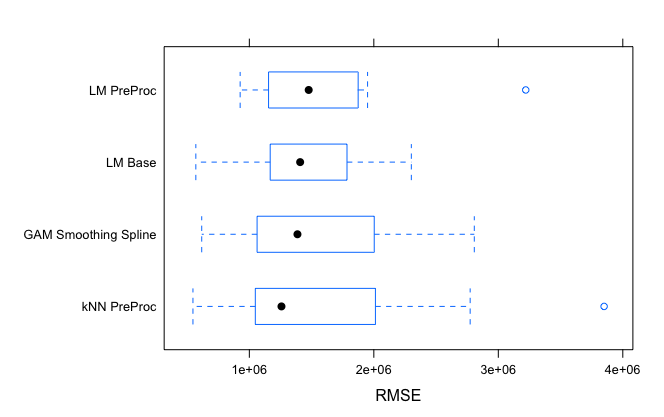
\includegraphics[scale=0.6]{images/train_RMSE_subset.png}
\label{fig:train_RMSE_sub}
\end{figure}

\begin{figure}[h!]
\centering
\caption{$R^2$ of species\_park\_subset Training Set}
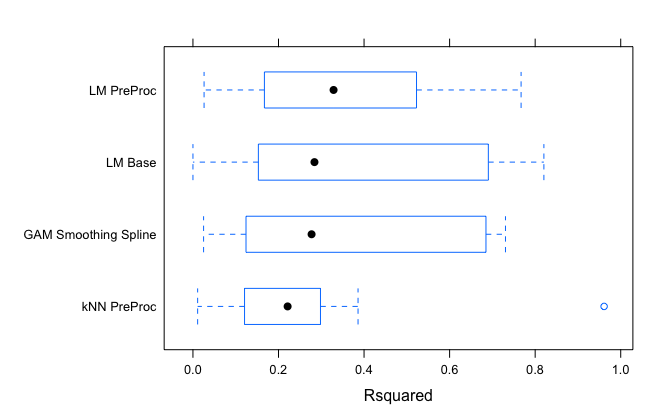
\includegraphics[scale=0.6]{images/train_R2_subset.png}
\label{fig:train_R2_sub}
\end{figure}

Next, the models were performed on the testing set. These results tell a different story compared to the results from the training set. Figure \ref{fig:test_RMSE_sub} shows kNN as the best fit model with the pre-processed linear regression following close by. However, the GAM smoothing spines and the base linear regression had the larger RMSE values. As for Figure \ref{fig:test_R2_sub}, kNN also had the best $R^2$ along with the pre-processed linear regression close behind. But just like the RMSE results, the GAM smoothing spline and the base linear regression were not so good and had small $R^2$ values. \\

Overall, even with the testing set's highest $R^2$ value at around 0.1, no significant conclusion can be made between the biodiversity at national parks and the number of visitors.

\begin{figure}[h!]
\centering
\caption{RMSE of species\_park\_subset Testing Set}
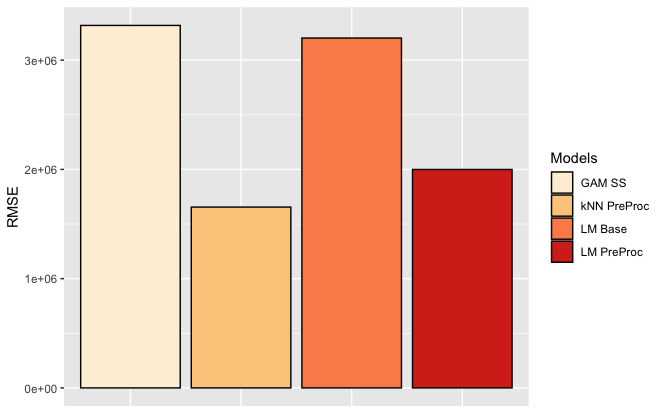
\includegraphics[scale=0.6]{images/test_RMSE_subset.png}
\label{fig:test_RMSE_sub}
\end{figure}

\begin{figure}[h!]
\centering
\caption{$R^2$ of species\_park\_subset Testing Set}
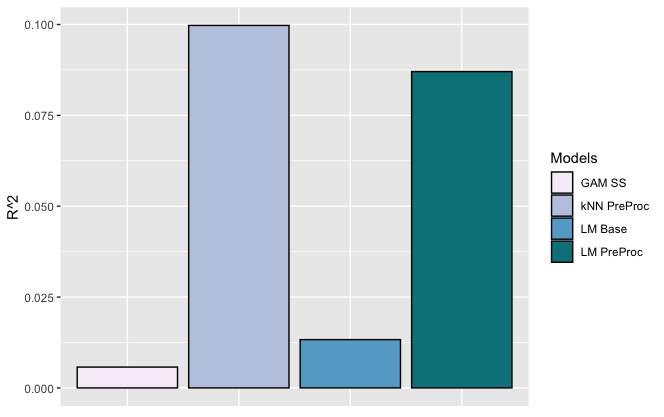
\includegraphics[scale=0.6]{images/test_R2_subset.png}
\label{fig:test_R2_sub}
\end{figure}

% SUBSECTION 4.1.1: LINEAR REGRESSION
\subsection{Linear Regression}
Table \ref{tab:lm} lists the different preliminary linear models created along with their AIC, $R^2$, and residual standard error (RSE).
\begin{table}[h!]
    \centering
    \caption{Preliminary Linear Regression Analysis on species\_parks\_subset}
    \begin{tabular}{c c c c}
    \hline
    \textbf{Linear Model} & \textbf{AIC} & \textbf{$R^2$} & \textbf{RSE} \\
    \hline
    Species+Acres &  1772.271 &  0.2294 & 1725000 \\
    Species & 1771.318 & 0.2294 & 1725000 \\
    Species+Acres+Species:Acres (Interaction Effect) & 1774.231 & 0.2151 & 1741000 \\
    \hline
    \end{tabular}
    \label{tab:lm}
\end{table}

The best model in this case is the linear regression model with only species. This model did better than the one with the interaction effect. Also, it did slightly better than the full model with acres because it had a smaller AIC value even though both of them had the same $R^2$ and RSE values.

% SUBSECTION 4.1.2: kNN
\subsubsection{kNN}
After running the kNN model, the number of neighbors that resulted in the smallest residual mean square error (RMSE) is nine. Overall, this model performed better than expected in the testing set with its low RMSE and high $R^2$.

% SUBSECTION 4.1.2: GAM SMOOTHING SPLINE
\subsubsection{GAM Smoothing Splines}
From using a 10-fold cross-validation, the two degrees of freedom resulted with the smallest RMSE. The training set did not provide much inference but the testing set showed that GAM smoothing spline is not the best model considering it had the lowest $R^2$ a and the highest RMSE.

%-----------------------------------------------------------------
% SUBSECTION 4.2: SPECIES ATTRIBUTES
\subsection{Species Attribute Analysis on Visitor Count}
The RMSE and $R^2$ of the training set are shown in Figure \ref{fig:train_RMSE_v2} and \ref{fig:train_R2_v2}. So far the RMSE boxplot displays the linear models as the best model, especially the model with only Seasonality and Abundance variables selected. Also, random forest and PLS is in the range with the linear models. From here on out the RMSE starts to increase for the PCR, lasso, ridge regression, and GAM smoothing spline models. As for the $R^2$ boxplot, LM PreProc, LM base, and GAM smoothing splines are shown as the best models. The other models however had a lower $R^2$ value.

\begin{figure}[h!]
\centering
\caption{RMSE of species\_parks\_v2 Training Set}
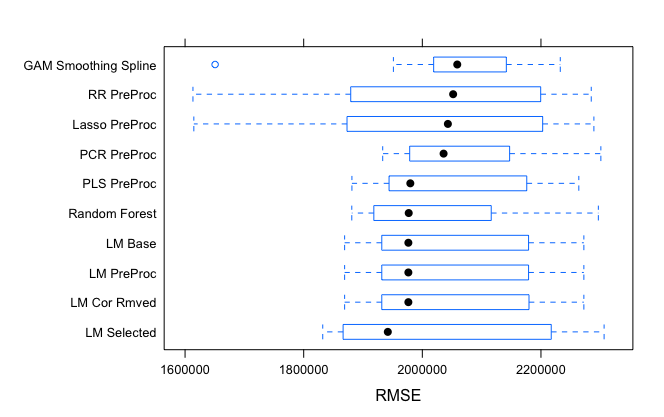
\includegraphics[scale=0.6]{images/train_RMSE_v2.png}
\label{fig:train_RMSE_v2}
\end{figure}

\begin{figure}[h!]
\centering
\caption{$R^2$ of species\_parks\_v2 Training Set}
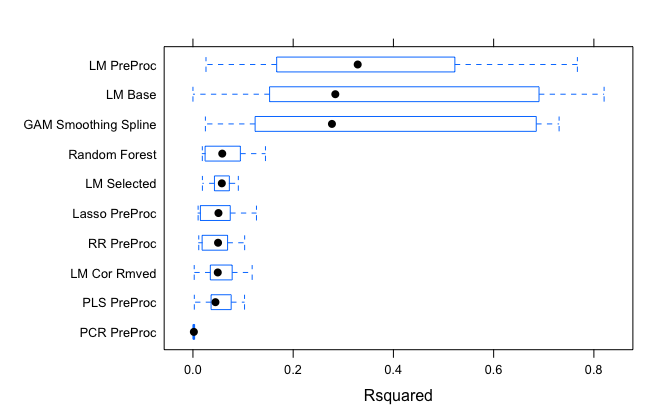
\includegraphics[scale=0.6]{images/train_R2_v2.png}
\label{fig:train_R2_v2}
\end{figure}

For the model's performance on the testing set, the results show the models to have about the same RMSE (Figure \ref{fig:test_RMSE_v2}), but their $R^2$ values (Figure \ref{fig:test_R2_v2}) are pretty varied. Random forest has the highest $R^2$ while PCR has the lowest, and most significant, $R^2$. The other models have about the same $R^2$ around 0.075 except GAM smoothing splines with 0.032. \\

Even with the testing set's highest $R^2$ value (< 0.125) not much inference can be made between the biodiversity of species and the number of visitors to these parks.

\begin{figure}[h!]
\centering
\caption{RMSE of species\_parks\_v2 Testing Set}
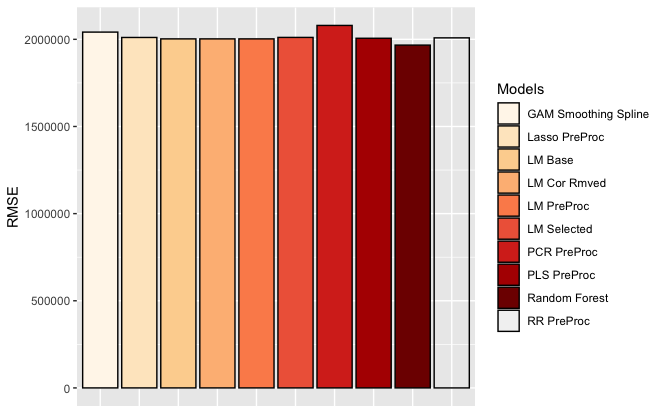
\includegraphics[scale=0.6]{images/test_RMSE_v2.png}
\label{fig:test_RMSE_v2}
\end{figure}

\begin{figure}[h!]
\centering
\caption{$R^2$ of species\_parks\_v2 Testing Set}
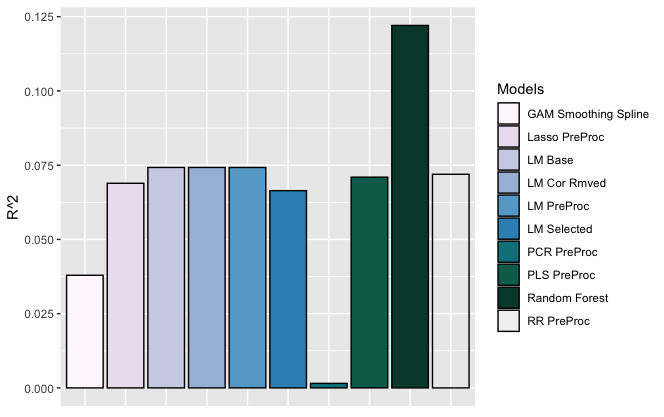
\includegraphics[scale=0.6]{images/test_R2_v2.png}
\label{fig:test_R2_v2}
\end{figure}

% SUBSECTION 4.2.1: LINEAR REGRESSION
\subsubsection{Linear Regression}
Based on Figure \ref{fig:train_RMSE_v2} and \ref{fig:train_R2_v2}, the LM Base and LM PreProc has been an overall good model, with a low RMSE and high $R^2$. The testing set though shows a different case (Figure \ref{fig:test_R2_v2}) . All the linear models did not perform as well as random forest but it did not perform as bad as PCR either.

% SUBSECTION 4.2.2: LASSO & RIDGE REGRESSION
\subsubsection{Ridge Regression \& Lasso}
After running the cv.glmnet function for ridge regression and lasso, the best lambda values are 28431.06 and 520498.2 respectively. Once the lambda values are applied to training set, its performance is pretty average in comparison to the other models. Applying lasso and ridge regression with their optimum lambda on the testing set too yielded similar results.

% SUBSECTION 4.2.3: PCR & PLS
\subsubsection{PCR \& PLS}
Based on Figure \ref{fig:train_RMSE_v2} and \ref{fig:train_R2_v2}, PCR and PLS would not be a good model considering they have a somewhat high RMSE and a low $R^2$. The caret function calculated the optimal principal component selected for PCR at one and for PLS at three. Applying these models and their optimum parameters to the testing set had PCR as the worse model, even with $R^2$ almost to zero (Figure \ref{fig:test_R2_v2}). The PLS was not as bad as the PCR. It yielded average results similar to the linear regression models.

% SUBSECTION 4.2.4: GAM SMOOTHING SPLINES
\subsubsection{GAM Smoothing Splines}
Figure \ref{fig:train_RMSE_v2} and \ref{fig:train_R2_v2} also shows GAM as a somewhat poor model since it has the highest RMSE. However, it did have a higher $R^2$ possibly due to the selected variables in the model being the only ones with significant coefficients. The optimal degrees of freedom selected for GAM smoothing splines from caret is one. Once these conditions are applied to the testing set, GAM smoothing splines still appears to be one of the lower performing models (Figure \ref{fig:test_R2_v2}).

% SUBSECTION 4.2.5: RANDOM FOREST
\subsubsection{Random Forest}
Figure \ref{fig:train_RMSE_v2} and \ref{fig:train_R2_v2} shows random forest did not perform as well as predicted. After finding the optimized number of trees at 100 with the best number of features at six, the model was neither good nor bad with respect to RMSE and $R^2$ values. As for the testing set, random forest perform pretty well as expected with the highest $R^2$ (Figure \ref{fig:test_R2_v2}).

%-----------------------------------------------------------------
% SECTION 5: DISCUSSION
\section{Discussion and Recommendations}
Overall, both linear models in species\_parks\_subset and species\_parks\_v2 exemplified the simplicity and power of the linear regression model especially after it has been pre-processed. It was predicted to be the worse model in the species\_parks\_v2 model, considering its multi-dimensionality, but based on the testing results it performed pretty well. \\

Another simple model that did better than expected is kNN. It was set as last place in the species\_parks\_subset dataset because of its drastic results when k changes. However, once caret found the optimized k neighbors, it kept at bay the bias-variance tradeoff and performed pretty well with the lowest RMSE and the highest $R^2$ out of the group. \\

One model that expectantly performed well is random forest. It is known to predict accurately for non-linear cases and can handle qualitative predictors, like in this case with the species\_parks\_v2 dataset. \\

Despite finding the best performing models on this dataset, it did not provide significant evidence of a relationship between biodiversity of national parks with the number of visitors. For further testing on this hypothesis, it will be simpler to focus on a handful of national parks first for preliminary analysis. Also, incorporating other features, other than biodiversity, can help provide a better picture on why people visit national parks and other ways to protect the area. Solely focusing on different species as the reason for people visiting national park is incomplete and may be affected by other unknown factors.

% REFERENCES
\printbibliography

\end{document}